\subsection{Cen�rio}

O uso da realidade aumentada em manuten��o de aeronaves pode trazer ganho no
fornecimento de informa��es de procedimentos, na previs�o de
falhas ou no reconhecimento de regi�es com falha.

 Como caso de uso ser� adotado a janela de inspe��o frontal, como mostrado na
 Figura~\ref{fig:ERJ190}, localizada na aeronave Embraer ERJ-190. 
 
\begin{figure}[h!]
\centering
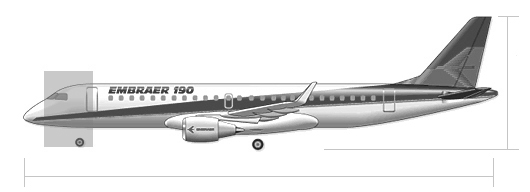
\includegraphics[scale=0.8]{images/ERJ190}
\caption{Posicionamento da janela de inspe��o. Fonte http://www.aero-news.net/}
\label{fig:ERJ190}
\end{figure}
